\chapter{Experimentos}
\thispagestyle{empty}

\section{Entorno de desarrollo}

El proyecto se llevó a cabo utilizando exclusivamente el lenguaje de programación \textit{Python} en su versión 3.11.8, debido a su versatilidad y eficacia en diversas áreas, desde el renderizado de modelos 3D en \textit{Blender} hasta el desarrollo de modelos de aprendizaje profundo. Se emplearon diversas bibliotecas para diferentes tareas: \textit{Trimesh} y \textit{PyVista} junto con \textit{VTK} para la manipulación de modelos 3D; \textit{Mediapipe} para la extracción de puntos de referencia faciales; \textit{NumPy} y \textit{pandas} para el procesamiento de datos; \textit{PIL} para el trabajo con imágenes; \textit{matplotlib} y \textit{Seaborn} para la generación de gráficos; \textit{Optuna} para la optimización de hiperparámetros; \textit{MLflow} para la gestión de experimentos; y, finalmente, \textit{PyTorch} en su versión 2.0.1 junto con las librerías CUDA para el entrenamiento de modelos de aprendizaje profundo.

Con el objetivo de realizar un control de versiones durante el desarrollo del proyecto, se utilizó Git junto con GitHub. El código generado se puede encontrar en el siguiente enlace \url{https://github.com/ivansalinasugr/TFG}. Para más información, consultar el Readme del repositorio.

\section{Entorno de ejecución}

El proceso de ejecución se lleva a cabo en un entorno de alto rendimiento ubicado en la Universidad de Granada, al que se accede de forma remota a través de SSH. Se emplea un script de Shell para configurar los parámetros esenciales de los archivos. Por un lado, se utiliza SLURM para reservar recursos en la partición \enquote*{dios} del clúster, asignando una GPU del nodo \enquote*{dionisio}. Este nodo cuenta con dos Quadro RTX 8000, una memoria RAM de 512 GB DDR4 y dos procesadores Intel Xeon Silver 4216. Por otro lado, Conda se encarga de gestionar el entorno de software, garantizando la disponibilidad de las bibliotecas necesarias durante el proceso.

\section{Resultados}

En este trabajo se realizarán varios experimentos para entrenar y validar los dos modelos de aprendizaje presentados en FacialSCDnet+. Antes de los entrenamientos, se llevará a cabo un ajuste de parámetros para optimizar el rendimiento de los modelos. Finalmente, se compararán los resultados obtenidos con los obtenidos en FacialSCDnet. Estas comparaciones se efectuarán mediante el rendimiento en dos conjuntos de imágenes: el conjunto de prueba sintético de FacialSCDnet+, y el conjunto real de FacialSCDnet. Esto nos permitirá evaluar la robustez y la capacidad de generalización de los modelos propuestos.

El objetivo de estos experimentos es validar la hipótesis de que los modelos presentados en este trabajo pueden igualar o superar el rendimiento del modelo de referencia y por tanto, estimar mejor la SCD en fotografías faciales. A continuación, se presentan los detalles específicos y los resultados de estos experimentos.


\subsection{Experimentos VGG-16}

Inicialmente, se llevó a cabo una fase de ajuste de hiperparámetros con el fin de determinar una configuración óptima para la arquitectura propuesta. Los rangos de valores y los parámetros finales se detallan en la Tabla \ref{hiper-vgg}. Además de los hiperparámetros mencionados, se estableció un entrenamiento a lo largo de 300 épocas, con una tasa de aprendizaje mínima de $10^{-12}$ y una reducción de la tasa de aprendizaje del 20\% cada 3 épocas consecutivas sin mejoras (paciencia), hasta un mínimo de $10^{-12}$.

\begin{table}[h]
	\centering
	\begin{tabular}{lll}
	\hline
	Parámetros          & Opciones                 & Mejor \\ \hline
	Optimizador         & {[}adam, sgd{]}          & adam  \\
	Tasa de aprendizaje & {[}$10^{-6}$, $10^{-3}${]}         & $4.63 \cdot 10^{-5}$      \\
	Tamaño del lote    & {[}16, 32, 64, 128{]}    & 32      \\
	Paciencia           & {[}2, 3, 4{]}            & 3     \\
	\textit{Early Stopping}     & {[}4, 6, 8{]}            & 6     \\
	\textit{Dropout} (\%)    & {[}0, 10, 20, 30{]} &  0 \\ \hline
	\end{tabular}
	\caption[Selección de parámetros de entrenamiento VGG-16.]{Parámetros de entrenamiento seleccionados para la red VGG-16, junto a los rangos de valores utilizados durante el proceso de optimización de hiperparámetros.}
	\label{hiper-vgg}
\end{table}

A continuación, la Figura \ref{fig30} muestra la gráfica de la función de pérdida durante el entrenamiento, mientras que la Tabla \ref{met-ent-vgg16} muestra los valores finales de las métricas tanto en el conjunto de entrenamiento como en el conjunto de validación.

\begin{figure}[h]
	\centering
	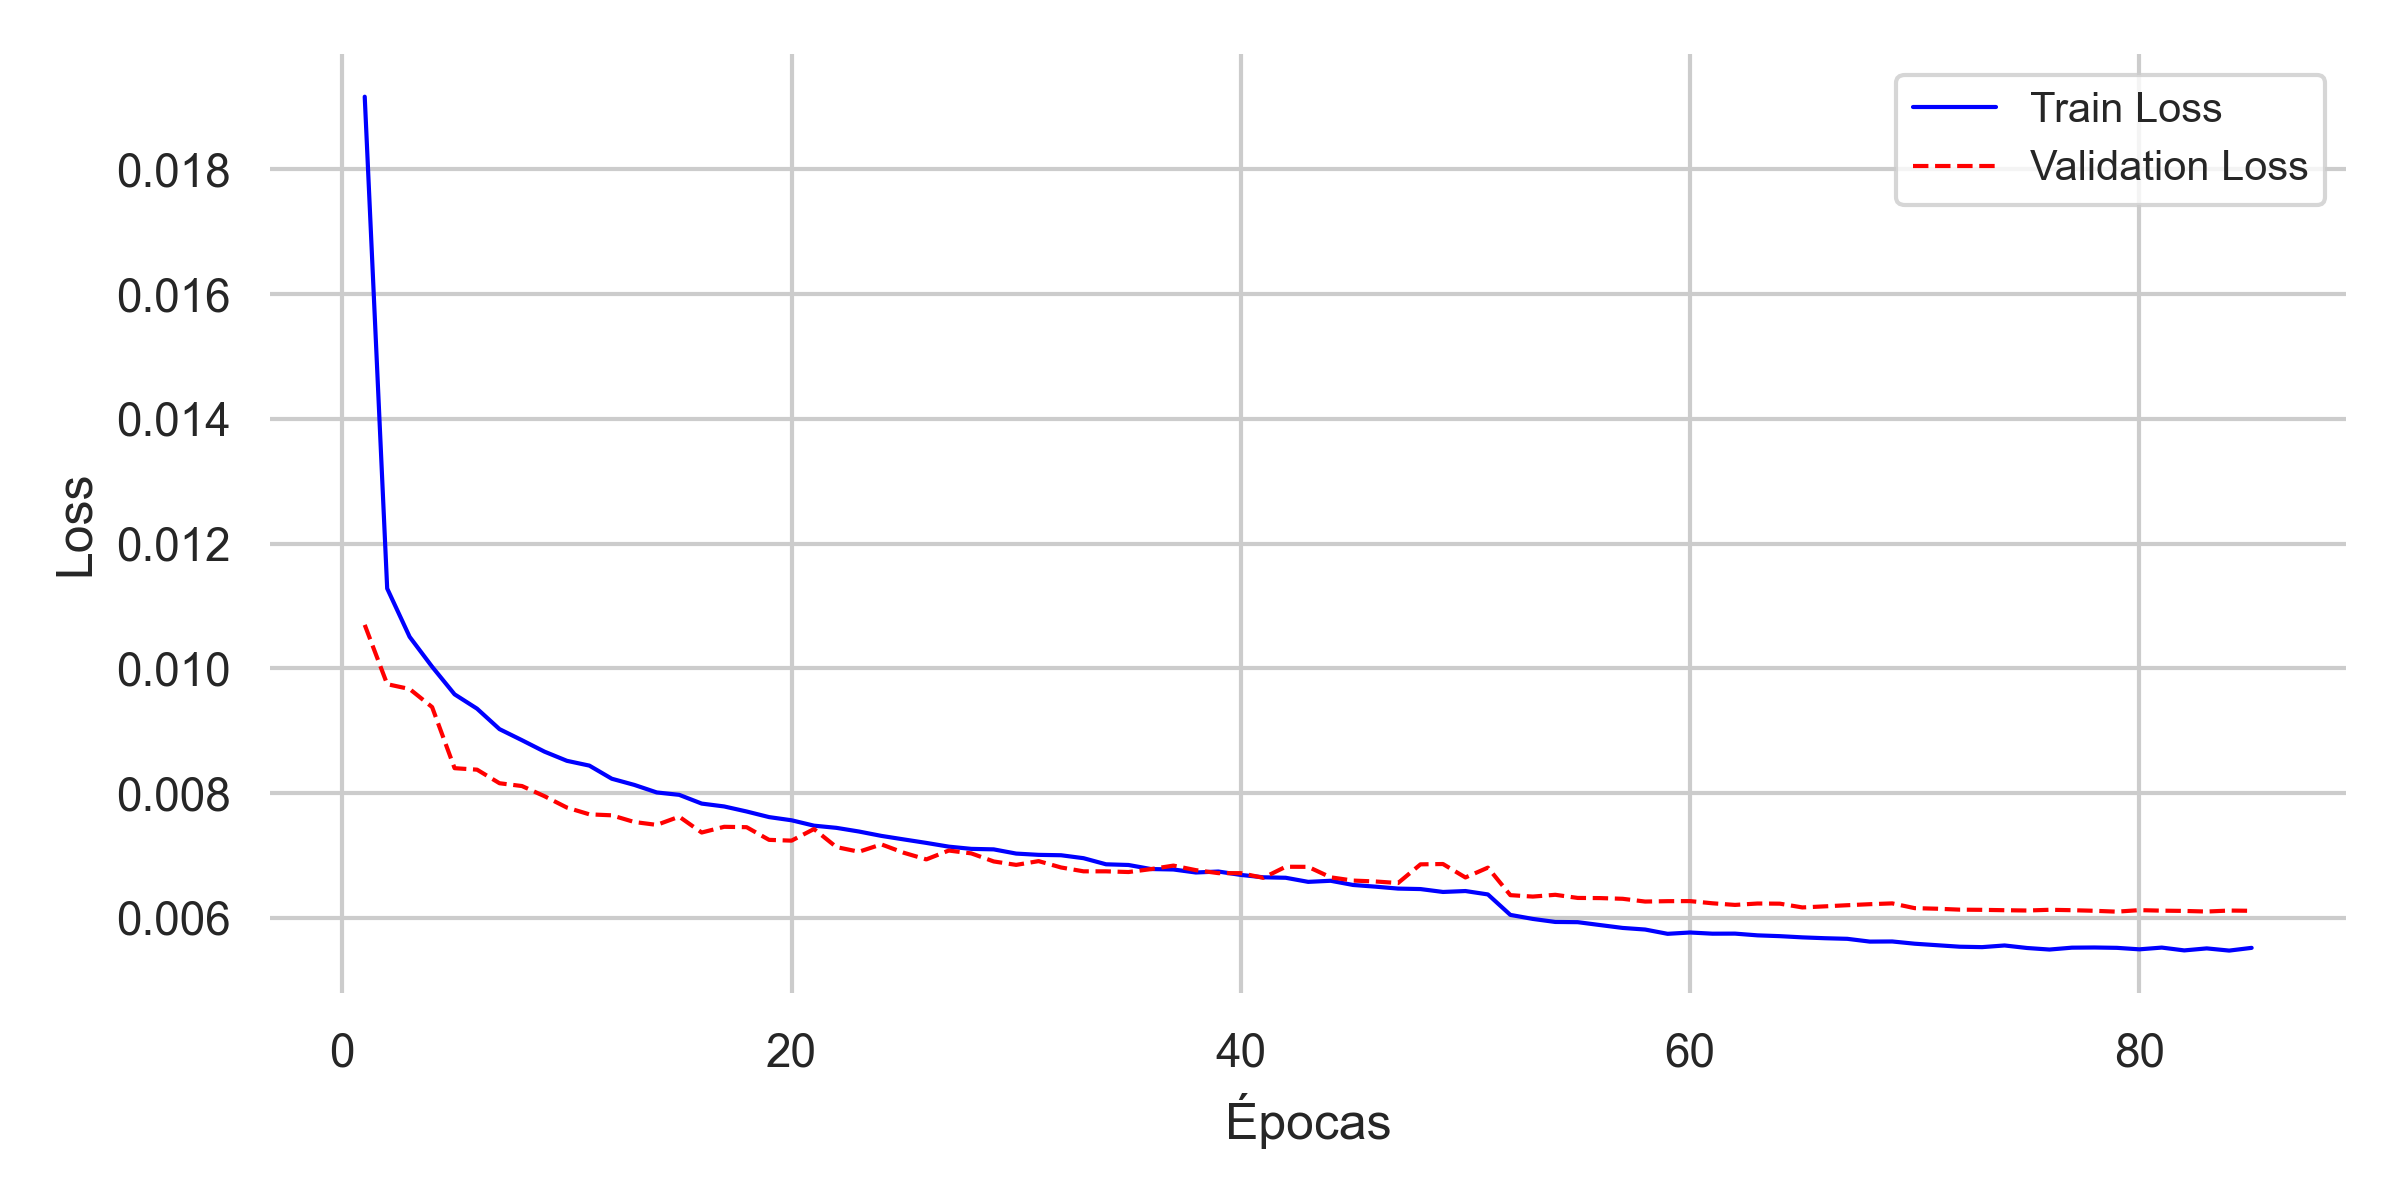
\includegraphics[scale=0.6]{imagenes/cap5/train_loss_vgg16.png}
	\caption[Gráfica de pérdida VGG-16.]{Gráfica de la función de pérdida durante el entrenamiento de la red VGG-16. En azul se representa la pérdida en el conjunto de entrenamiento mientras que en naranja se representa la pérdida en el conjunto de validación.}
	\label{fig30}
\end{figure}

Al inicio del entrenamiento, se observa un descenso pronunciado en ambas curvas de pérdida, lo que indica un aprendizaje rápido del modelo. A medida que avanzan las épocas, ambas curvas comienzan a estabilizarse. La pérdida en el entrenamiento continúa disminuyendo, aunque a un ritmo más lento, sugiriendo que el modelo sigue ajustando sus parámetros, pero con mejoras incrementales más pequeñas. La curva de validación también desciende inicialmente y luego se estabiliza. Sin embargo, en las últimas épocas, esta pérdida se mantiene prácticamente constante o presenta pequeñas fluctuacione, indicando que el modelo no mejora significativamente en términos de generalización más allá de cierto punto.

Después de seis épocas sin mejorar en validación, se produce el \textit{early stopping}. La aplicación de esta técnica parece haber sido efectiva, ya que no se observa una gran divergencia entre las pérdidas de entrenamiento y validación hacia el final de la gráfica. Esto indica que el modelo no está sobreajustando significativamente y mantiene un buen equilibrio entre el ajuste a los datos de entrenamiento y su capacidad de generalización.

\begin{table}[h]
	\centering
	\resizebox{\textwidth}{!}{%
	\begin{tabular}{llll}
	\hline
	Métricas de evaluación &
	   &
	  Entrenamiento &
	  Validación \\ \hline
	Distorsión &
	  \begin{tabular}[c]{@{}l@{}}Media (std)\\ Mediana\\ Mínimo\\ Perc 90, 95, 99\end{tabular} &
	  \begin{tabular}[c]{@{}l@{}}0.005 (0.004)\\ 0.003\\ 0.0\\ {[}0.01, 0.013, 0.02{]}\end{tabular} &
	  \begin{tabular}[c]{@{}l@{}}0.006 (0.006)\\ 0.004\\ 0.0\\ {[}0.014, 0.017, 0.027{]}\end{tabular} \\ \hline
	MAE (cm) &
	  \begin{tabular}[c]{@{}l@{}}Media (std)\\ Mediana\\ Mínimo\\ Perc 90, 95, 99\end{tabular} &
	  \begin{tabular}[c]{@{}l@{}}24.696 (35.699)\\ 9.258\\ 0.0\\ {[}70.687, 100.423, 164.784{]}\end{tabular} &
	  \begin{tabular}[c]{@{}l@{}}31.425 (44.048)\\ 12.194\\ 0.0\\ {[}89.95, 125.105, 204.385{]}\end{tabular} \\ \hline
	MRE (\%) &
	  \begin{tabular}[c]{@{}l@{}}Media (std)\\ Mediana\\ Mínimo\\ Perc 90, 95, 99\end{tabular} &
	  \begin{tabular}[c]{@{}l@{}}0.085 (0.103)\\ 0.057\\ 0.0\\ {[}0.183, 0.254, 0.487{]}\end{tabular} &
	  \begin{tabular}[c]{@{}l@{}}0.111 (0.138)\\ 0.075\\ 0.0\\ {[}0.233, 0.328, 0.647{]}\end{tabular} \\ \hline
	\end{tabular}%
	}
	\caption[Métricas en entrenamiento y validación VGG-16.]{Métricas en los conjuntos de entrenamiento y de validación tras el proceso de entrenamiento de la red VGG-16.}
	\label{met-ent-vgg16}
\end{table}

La tabla \ref{met-ent-vgg16} proporciona un análisis detallado de las métricas de evaluación del modelo VGG-16 en los conjuntos de entrenamiento y validación. Al observar estas métricas, se pueden extraer las siguientes conclusiones:

\begin{itemize}
	\item Distorsión: La distorsión media es próxima a cero en ambos conjuntos, con valores muy cercanos entre sí, lo que indica que el modelo mantiene una consistencia adecuada entre las predicciones de los datos de entrenamiento y validación. La desviación estándar es ligeramente mayor en la validación, sugiriendo una pequeña variabilidad adicional en este conjunto. Los percentiles muestran que, aunque en general los valores son bajos, la distorsión en los casos extremos es ligeramente mayor en el conjunto de validación.
	\item Error absoluto medio: La media del MAE es considerablemente mayor en la validación comparado con el entrenamiento, lo que indica que el modelo tiene un mejor rendimiento en términos de precisión en el conjunto de entrenamiento. La mediana del MAE también es menor en el entrenamiento, lo que refuerza la idea de un mejor rendimiento en este conjunto. Sin embargo, la presencia de valores de MAE más altos en los percentiles superiores del conjunto de validación sugiere que existen algunas predicciones con errores significativos en este conjunto.
	\item Error relativo medio: El MRE promedio es bajo en ambos conjuntos, pero es mayor en la validación en comparación con el entrenamiento. La mediana y los percentiles superiores del MRE también son mayores en la validación, lo que implica que, aunque la mayoría de los errores relativos son pequeños, los peores casos de error relativo son más severos en el conjunto de validación.
\end{itemize}

En general, aunque la precisión es mayor en el conjunto de entrenamiento en comparación con el de validación, las métricas indican que el modelo VGG-16 ha sido entrenado de manera efectiva, con buenos resultados generales y una adecuada aplicación de técnicas de prevención del sobreajuste.

\subsection{Experimentos ResNet-50}

Al igual que con VGG-16, primero se llevó a cabo una fase de ajuste de hiperparámetros con el fin de determinar una configuración óptima para la arquitectura propuesta. Los rangos de valores y los parámetros finales se detallan en la Tabla \ref{hiper-resnet}. Además de los hiperparámetros mencionados, se estableció un entrenamiento a lo largo de 300 épocas, con una tasa de aprendizaje mínima de $10^{-12}$ y una reducción de la tasa de aprendizaje del 20\% cada 3 épocas consecutivas sin mejoras (paciencia), hasta un mínimo de $10^{-12}$.

\begin{table}[h]
	\centering
	\begin{tabular}{lll}
	\hline
	Parámetros          & Opciones                 & Mejor \\ \hline
	Optimizador         & {[}adam, sgd{]}          &  adam \\
	Tasa de aprendizaje & {[}$10^{-6}$, $10^{-3}${]}  &  0.00042  \\
	Tamaño del lote     & {[}16, 32, 64, 128{]}    &  32     \\
	Paciencia           & {[}2, 3, 4{]}            &  3   \\
	Parada temprana     & {[}4, 6, 8{]}            &  6   \\
	\textit{Dropout} (\%)    & {[}0, 10, 20, 30{]} &  0  \\ \hline
	\end{tabular}
	\caption[Selección de parámetros de entrenamiento ResNet-50.]{Parámetros de entrenamiento seleccionados para la red ResNet-50, junto a los rangos de valores utilizados durante el proceso de optimización de hiperparámetros.}
	\label{hiper-resnet}
\end{table}

A continuación, la Figura \ref{fig31} muestra la gráfica de la función de pérdida durante el entrenamiento, mientras que la Tabla \ref{met-ent-resnet} muestra los valores finales de las métricas.

\begin{figure}[h]
	\centering
	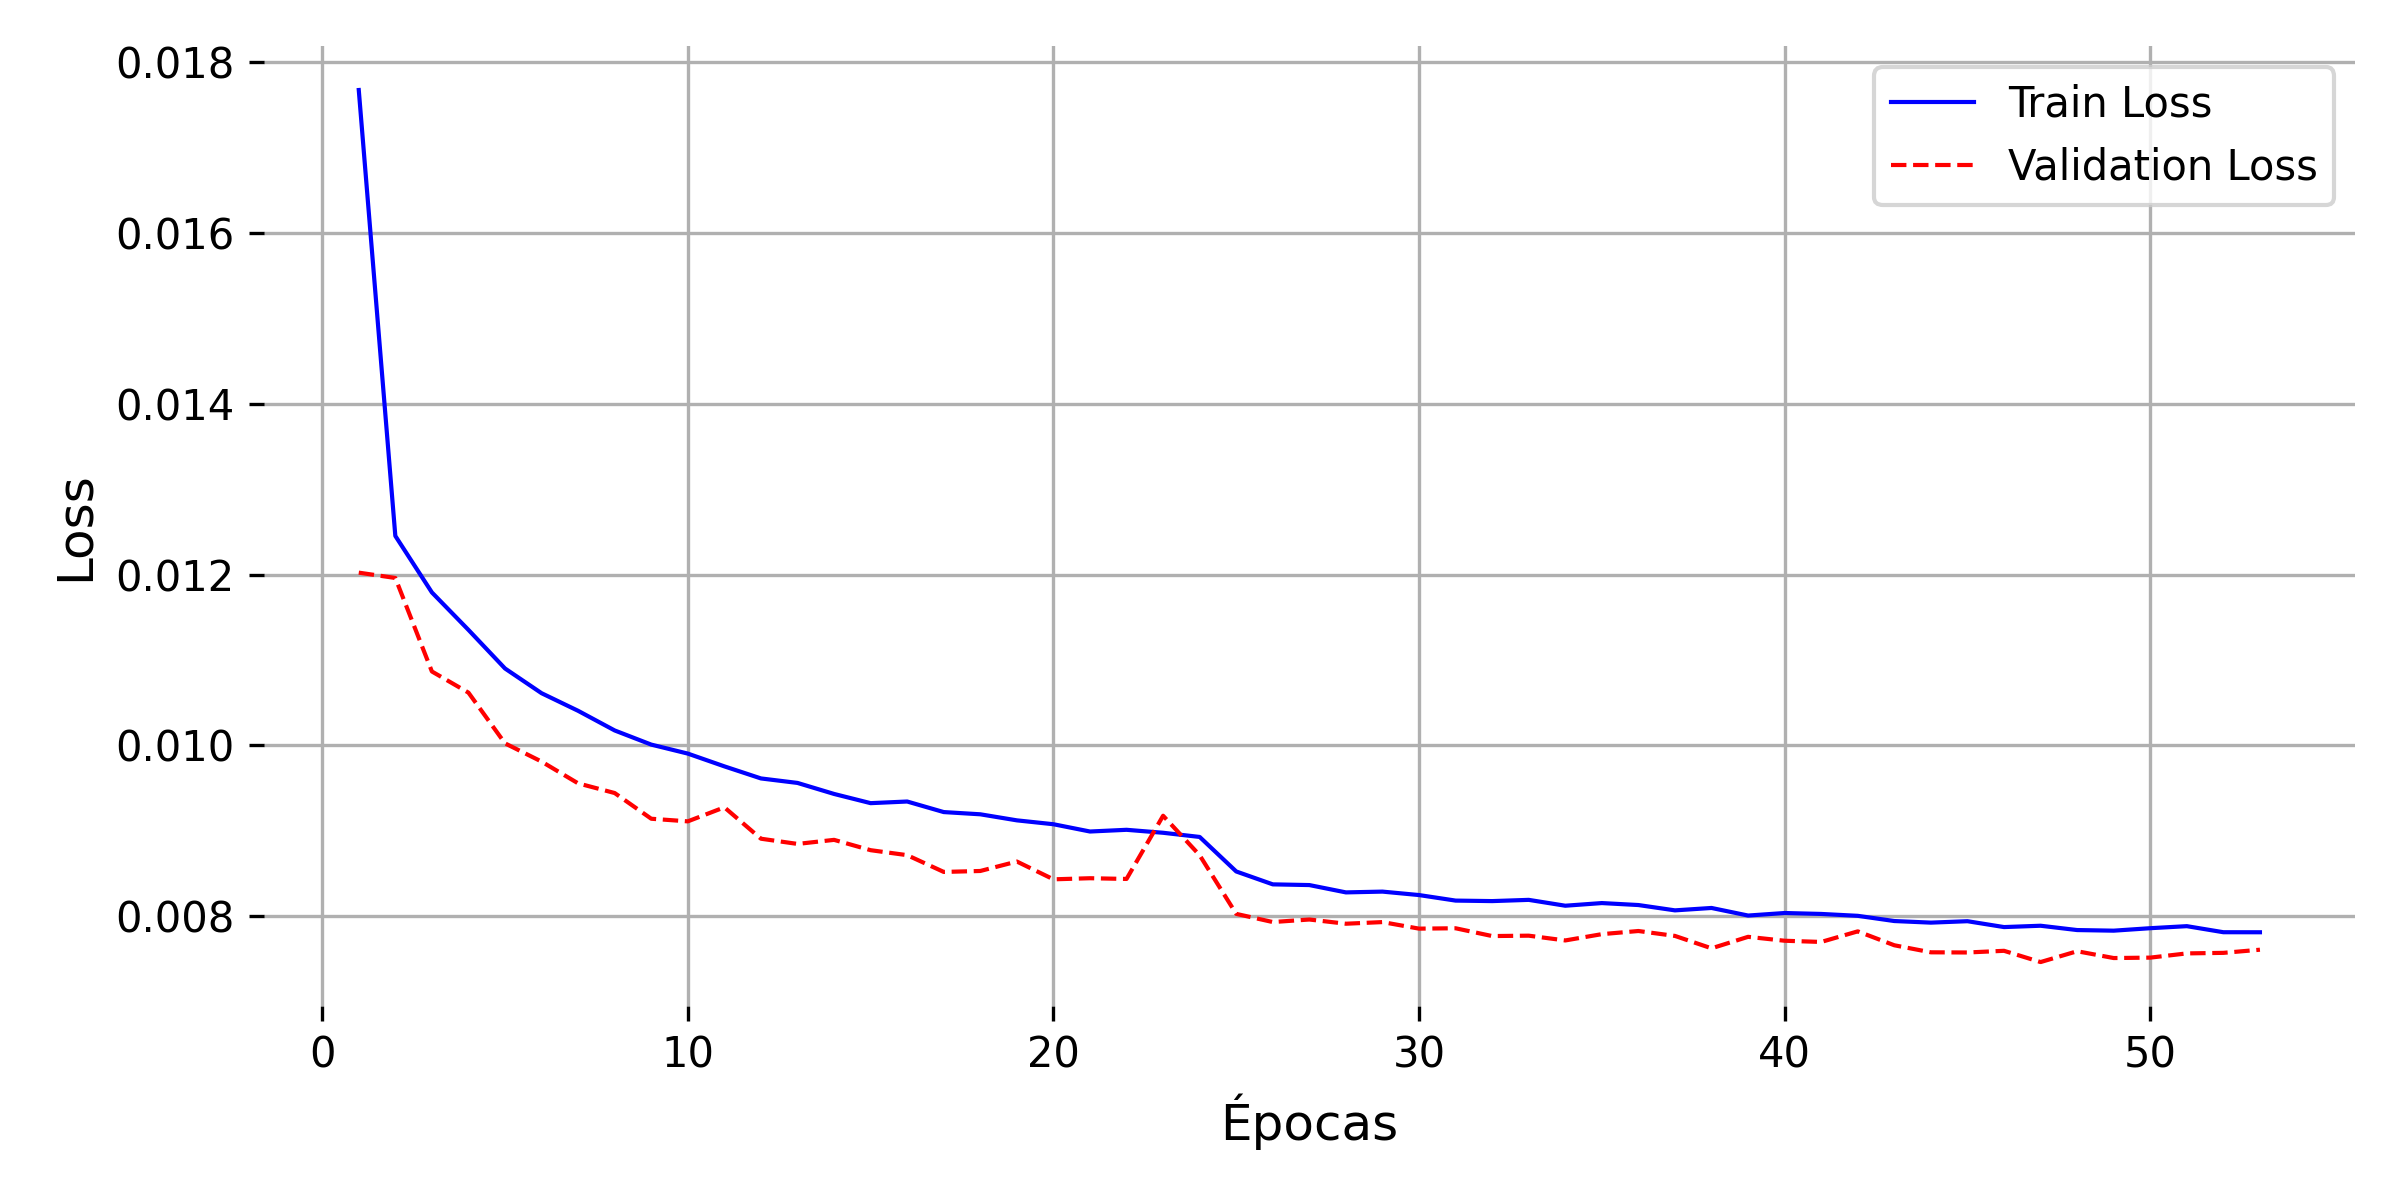
\includegraphics[scale=0.6]{imagenes/cap5/train_loss_resnet.png}
	\caption[Gráfica de pérdida ResNet-50.]{Gráfica de la función de pérdida durante el entrenamiento de la red ResNet-50. En azul se representa la pérdida en el conjunto de entrenamiento mientras que en naranja se representa la pérdida en el conjunto de validación.}
	\label{fig31}
\end{figure}

Al inicio del entrenamiento, ambas curvas de pérdida muestran un descenso pronunciado, lo que indica que el modelo está aprendiendo rápidamente y ajustando sus parámetros de manera eficiente durante las primeras épocas. A partir de aproximadamente la décima época, el descenso de la función de pérdida se ralentiza, sugiriendo que el modelo está entrando en una fase de refinamiento donde las mejoras son más incrementales. Tanto la pérdida de entrenamiento como la de validación continúan disminuyendo, aunque a un ritmo más lento. Hacia el final del entrenamiento, las curvas de pérdida de entrenamiento y validación convergen y se vuelven muy cercanas entre sí. Es en este punto cuando se estabiliza la pérdida en validación y se produce el \textit{early stopping}.

El hecho de que ambas pérdidas estén tan próximas es un buen indicio de que el modelo no está sobreajustando y está manteniendo su capacidad de generalización. Sin embargo, el modelo podría ajustarse mejor a los datos, ya que la curva de entrenamiento apenas decrece en las últimas épocas.

\begin{table}[h]
	\centering
	\resizebox{\textwidth}{!}{%
	\begin{tabular}{llll}
	\hline
	Métricas de evaluación &
	&
	Entrenamiento &
	Validación \\ \hline
	Distorsión &
	\begin{tabular}[c]{@{}l@{}}Media (std)\\ Mediana\\ Mínimo\\ Perc 90, 95, 99\end{tabular} &
	\begin{tabular}[c]{@{}l@{}}0.007 (0.007)\\ 0.005\\ 0.0\\ {[}0.016, 0.02, 0.031{]}\end{tabular} &
	\begin{tabular}[c]{@{}l@{}}0.007 (0.007)\\ 0.005\\ 0.0\\ {[}0.017, 0.022, 0.033{]}\end{tabular} \\ \hline
	MAE (cm) &
	\begin{tabular}[c]{@{}l@{}}Media (std)\\ Mediana\\ Mínimo\\ Perc 90, 95, 99\end{tabular} &
	\begin{tabular}[c]{@{}l@{}}31.142 (40.425)\\ 14.228\\ 0.0\\ {[}85.653, 117.846, 183.365{]}\end{tabular} &
	\begin{tabular}[c]{@{}l@{}}34.072 (43.447)\\ 15.597\\ 0.002\\ {[}93.849, 126.878, 194.479{]}\end{tabular} \\ \hline
	MRE (\%) &
	\begin{tabular}[c]{@{}l@{}}Media (std)\\ Mediana\\ Mínimo\\ Perc 90, 95, 99\end{tabular} &
	\begin{tabular}[c]{@{}l@{}}0.117 (0.125)\\ 0.085\\ 0.0\\ {[}0.245, 0.327, 0.581{]}\end{tabular} &
	\begin{tabular}[c]{@{}l@{}}0.128 (0.137)\\ 0.093\\ 0.0\\ {[}0.266, 0.356, 0.659{]}\end{tabular} \\ \hline
	\end{tabular}%
	}
	\caption[Métricas en entrenamiento y validación ResNet-50.]{Métricas en los conjuntos de entrenamiento y de validación tras el proceso de entrenamiento de la red ResNet-50.}
	\label{met-ent-resnet}
\end{table}

La tabla \ref{met-ent-resnet} proporciona un análisis detallado de las métricas de evaluación del modelo ResNet-50 en los conjuntos de entrenamiento y validación. Al observar estas métricas, se pueden extraer las siguientes conclusiones:

\begin{itemize}
	\item Distorsión: La distorsión media es igual en ambos conjuntos, con desviaciones estándar idénticas, lo que indica una consistencia adecuada entre las prediciones de los datos de entrenamiento y validación. La mediana es también baja en ambos conjuntos. Los percentiles muestran valores ligeramente mayores en la validación, sugiriendo que en los casos extremos la distorsión es algo mayor en este conjunto.
	\item Error absoluto medio: La media del MAE es mayor en la validación comparado con el entrenamiento, indicando que el modelo tiene un mejor rendimiento en términos de precisión en el conjunto de entrenamiento. La mediana del MAE también es menor en el entrenamiento en comparación con la validación. Los percentiles superiores del MAE son más altos en la validación, lo que sugiere la presencia de predicciones con errores significativos en este conjunto.
	\item Error relativo medio: El MRE promedio es bajo en ambos conjuntos, pero ligeramente mayor en la validación en comparación con el entrenamiento. La mediana y los percentiles superiores del MRE también son mayores en la validación, lo que implica que, aunque la mayoría de los errores relativos son pequeños, los peores casos de error relativo son más severos en el conjunto de validación.
\end{itemize}

En general, aunque la precisión es mayor en el conjunto de entrenamiento en comparación con el de validación, las métricas indican que el modelo ResNet-50 ha sido entrenado de manera efectiva, con buenos resultados generales y una adecuada aplicación de técnicas de prevención del sobreajuste.


\subsection{Comparación FacialSCDnet}

En esta sección se lleva a cabo una comparativa entre los tres modelos utilizados para la estimación de la SCD: VGG-16 de FacialSCDnet, VGG-16 de FacialSCDnet+ y ResNet-50 de FacialSCDnet+. Para ello, se evalúan los modelos en dos conjuntos de datos: el conjunto de datos sintético de FacialSCDnet+, previamente definido en la Sección \ref{protocolo}, y el conjunto de datos de imágenes reales utilizado en FacialSCDnet.

Para hacer la comparación más visual, se complementarán las métricas con figuras que muestren las predicciones comparadas con los valores objetivo, así como los errores de predicción representados en diagramas de caja y de violín.

\subsubsection{Test con imágenes FacialSCDnet+}

Este conjunto de datos contiene 28935 imágenes sintéticas en 35 distancias desde 50 a 600 cm. Los resultados de evaluar los modelos en este conjunto de datos se muestran en la Tabla \ref{test-mio}.

\begin{table}[h]
	\centering
	\resizebox{\textwidth}{!}{%
	\begin{tabular}{lllll}
	\hline
	\begin{tabular}[c]{@{}l@{}}Métricas de \\ evaluación\end{tabular} &
	   &
	  \begin{tabular}[c]{@{}l@{}}VGG-16 \\ FacialSCDnet\end{tabular} &
	  \begin{tabular}[c]{@{}l@{}}VGG-16 \\ FacialSCDnet+\end{tabular} &
	  \begin{tabular}[c]{@{}l@{}}ResNet-50 \\ FacialSCDnet+\end{tabular} \\ \hline
	Distorsión &
	  \begin{tabular}[c]{@{}l@{}}Media (std)\\ Mediana\\ Mínimo\\ Perc 90\\ Perc 95\\ Perc 99\end{tabular} &
	  \begin{tabular}[c]{@{}l@{}}0.012 (0.014)\\ 0.008\\ 0.0\\ 0.029\\ 0.039\\ 0.068\end{tabular} &
	  \begin{tabular}[c]{@{}l@{}}0.006 (0.006)\\ 0.005\\ 0.0\\ 0.014\\ 0.018\\ 0.026\end{tabular} &
	  \begin{tabular}[c]{@{}l@{}}0.008 (0.008)\\ 0.006\\ 0.0\\ 0.018\\ 0.023\\ 0.034\end{tabular} \\ \hline
	MAE (cm) &
	  \begin{tabular}[c]{@{}l@{}}Media (std)\\ Mediana\\ Mínimo\\ Perc 90\\ Perc 95\\ Perc 99\end{tabular} &
	  \begin{tabular}[c]{@{}l@{}}53.237 (73.434)\\ 21.594\\ 0.003\\ 147.604\\ 220.045\\ 338.481\end{tabular} &
	  \begin{tabular}[c]{@{}l@{}}32.165 (44.045)\\ 12.771\\ 0.0\\ 92.037\\ 127.188\\ 200.072\end{tabular} &
	  \begin{tabular}[c]{@{}l@{}}35.095 (43.954)\\ 16.498\\ 0.001\\ 96.793\\ 130.565\\ 193.916\end{tabular} \\ \hline
	MRE (\%) &
	  \begin{tabular}[c]{@{}l@{}}Media (std)\\ Mediana\\ Mínimo\\ Perc 90\\ Perc 95\\ Perc 99\end{tabular} &
	  \begin{tabular}[c]{@{}l@{}}0.215 (0.299)\\ 0.132\\ 0.0\\ 0.455\\ 0.681\\ 1.567\end{tabular} &
	  \begin{tabular}[c]{@{}l@{}}0.113 (0.135)\\ 0.078\\ 0.0\\ 0.24\\ 0.327\\ 0.64\end{tabular} &
	  \begin{tabular}[c]{@{}l@{}}0.133 (0.14)\\ 0.099\\ 0.0\\ 0.277\\ 0.362\\ 0.669\end{tabular} \\ \hline
	\end{tabular}%
	}
	\caption[Métricas en el conjunto de test de FacialSCDnet+.]{Métricas en el conjunto de test de FacialSCDnet+, comparando los modelos VGG-16 y ResNet-50 de FacialSCDnet+ contra el modelo de FacialSCDnet.}
	\label{test-mio}
\end{table}

Esta tabla refleja cómo VGG-16 FacialSCDnet+ presenta mejores resultados en la mayoría de las métricas, seguido por ResNet-50 FacialSCDnet+ y VGG-16 FacialSCDnet. Estos resultados sugieren que el método FacialSCDnet+ proporciona una mejora significativa en el rendimiento de la predicción en comparación con el método FacialSCDnet estándar, y que el modelo VGG-16, especialmente con el método FacialSCDnet+, es más efectivo que el ResNet-50 en este contexto específico.

Estos resultados, en teoría, son lo esperado, ya que los modelos de FacialSCDnet+ han sido entrenados en un conjunto similar al que se está utilizando para el test, mientras que el modelo FacialSCDnet fue entrenado con un conjunto diferente.

La siguiente gráfica (Figura \ref{fig32}) muestra los valores predichos frente a los valores objetivos para cada uno de los 3 modelos utilizados. La línea roja discontinua representa la línea de referencia donde las predicciones coincidirían perfectamente con las etiquetas objetivo. 

\begin{figure}[h]
	\centering
	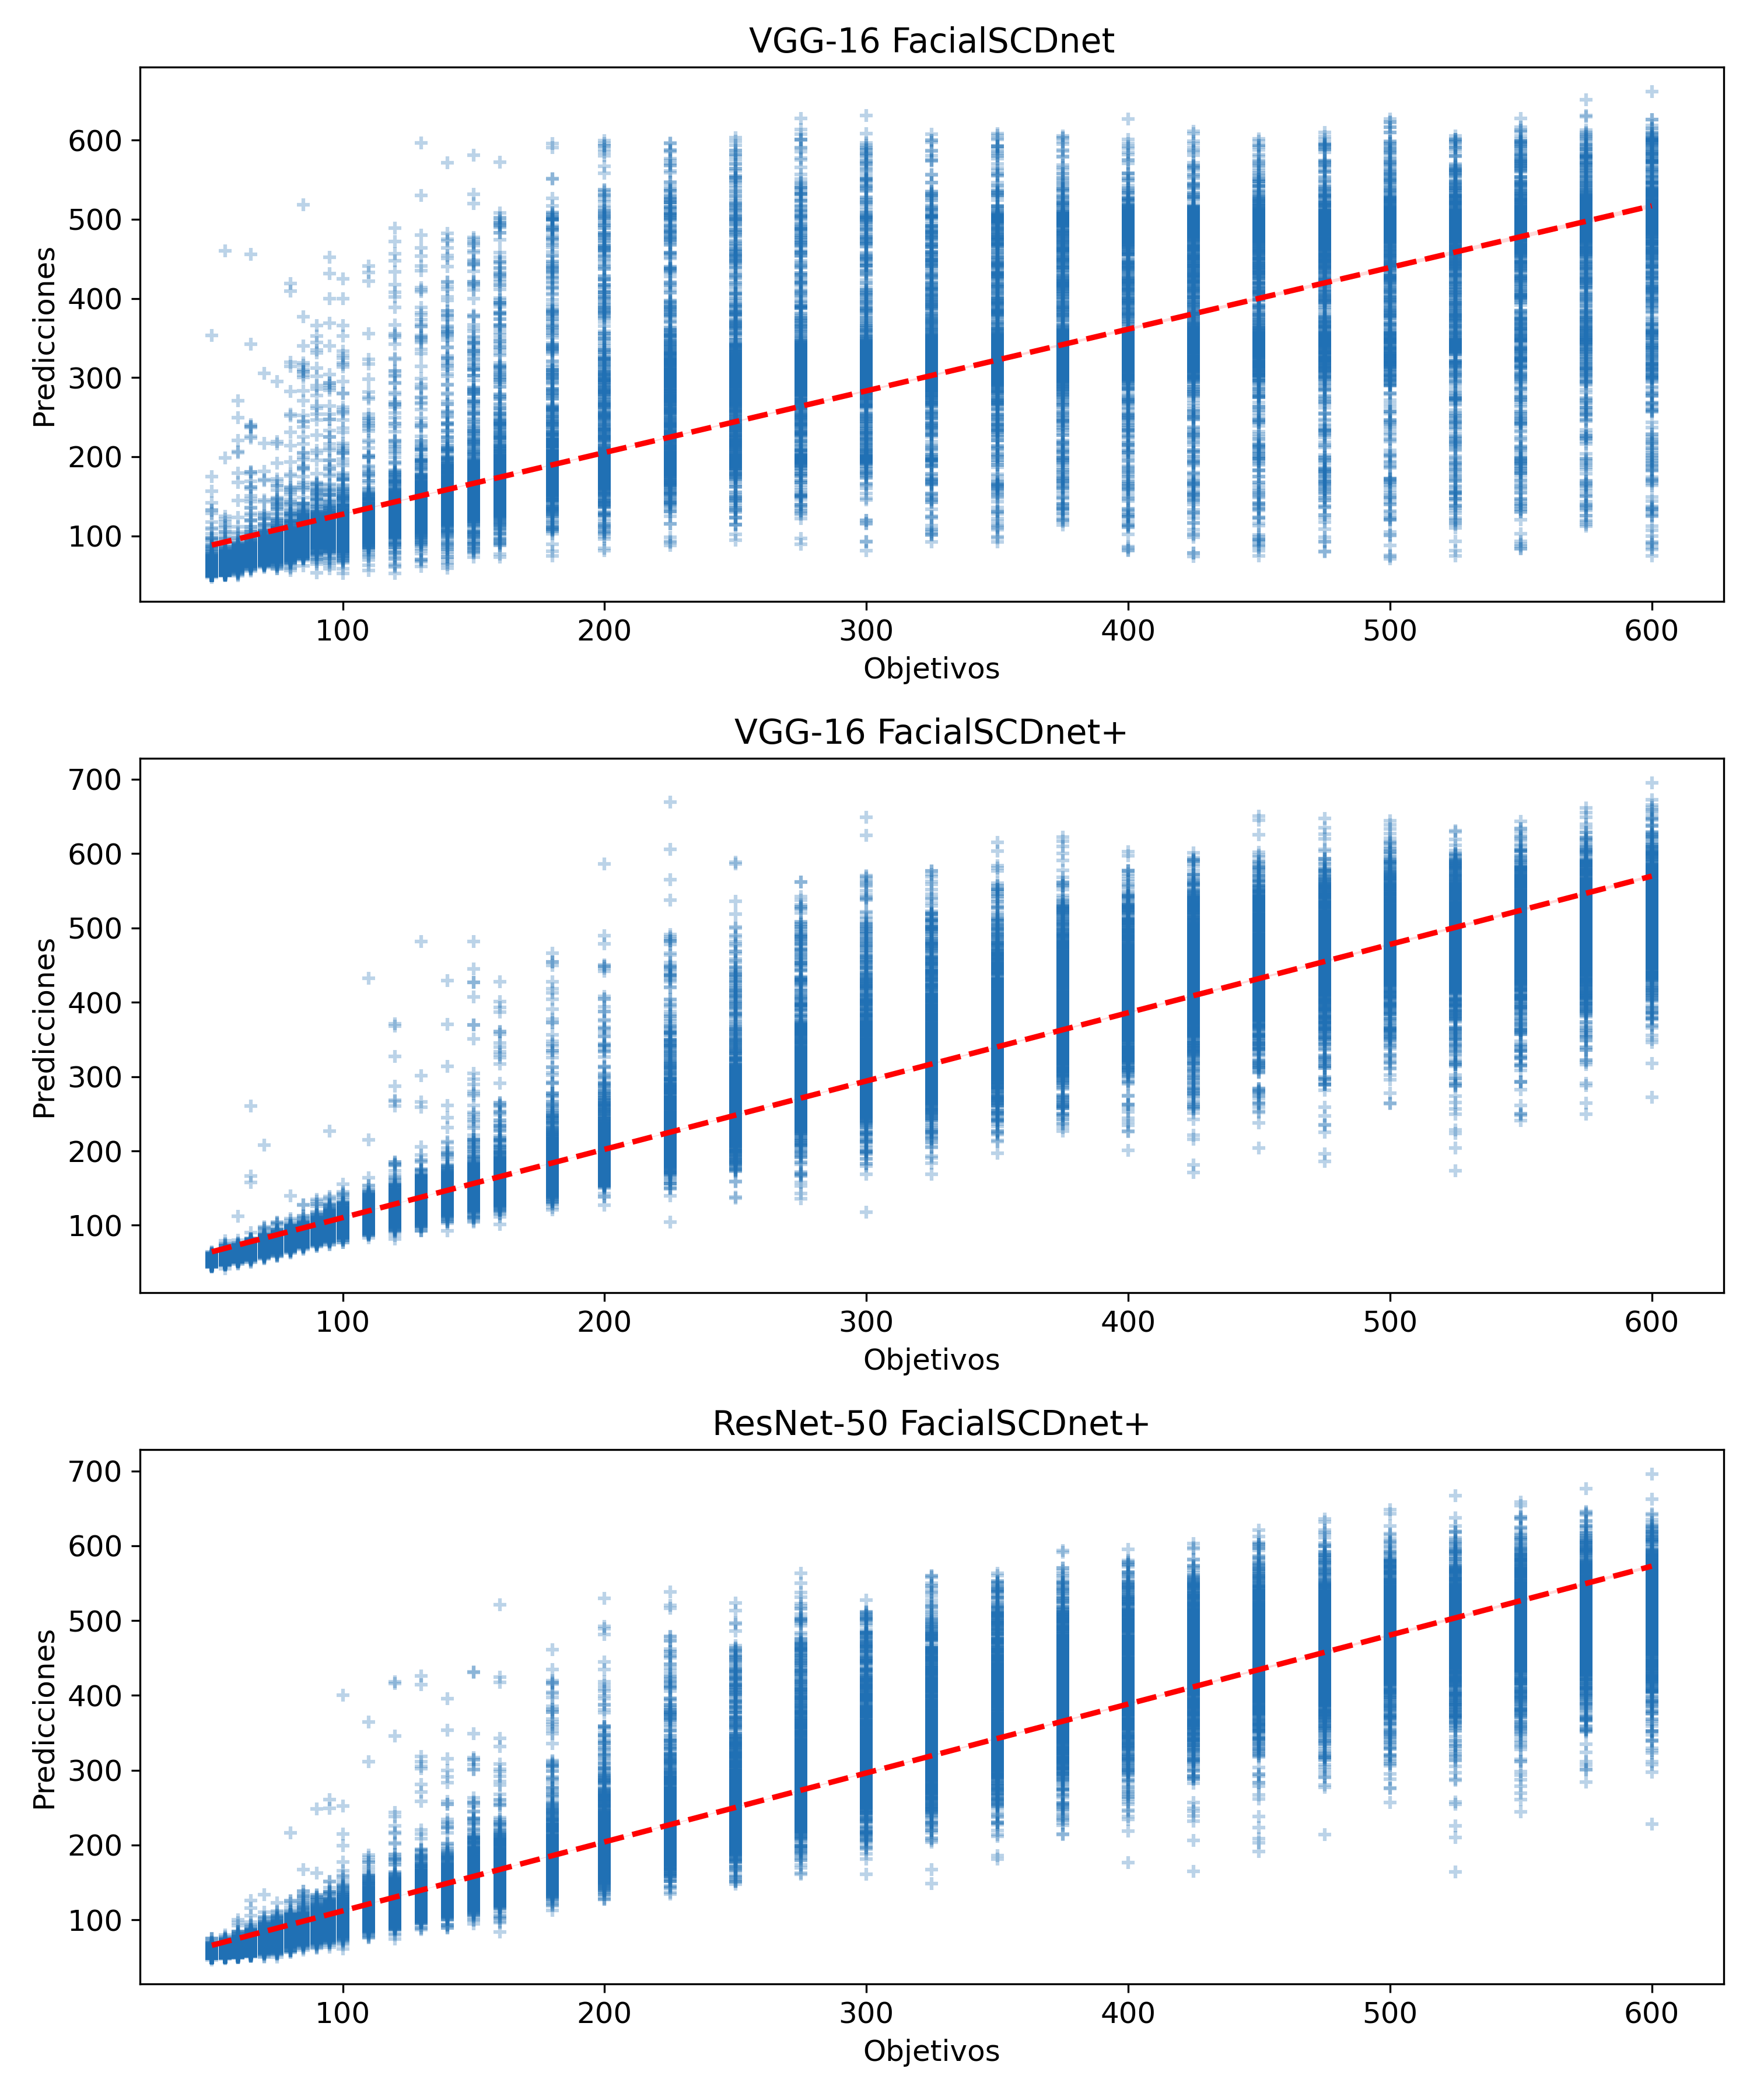
\includegraphics[width=\textwidth]{imagenes/cap5/comp_etiquetas_own.png}
	\caption[Comparación etiquetas test FacialSCDnet+.]{Gráfica que muestra la comparación de etiquetas predichas vs las etiquetas objetivo para cada uno de los 3 modelos utilizados.}
	\label{fig32}
\end{figure}

Se observa como en el modelo VGG-16 FacialSCDnet las predicciones son mucho más érroneas tanto a distancias cortas como largas, en comparación con los otros dos modelos. Los modelos FacialSCDnet+ predicen mejor, especialmente a distancias cortas, aunque también superan a FacialSCDnet en distancias largas. En particular, el modelo VGG-16 FacialSCDnet+ muestra un desempeño excepcionalmente bueno a cortas distancias.

La figura \ref{fig33} muestra una comparación de las predicciones de error para los tres modelos utilizando tanto gráficos de caja como gráficos de violín.

\begin{figure}[h]
	\centering
	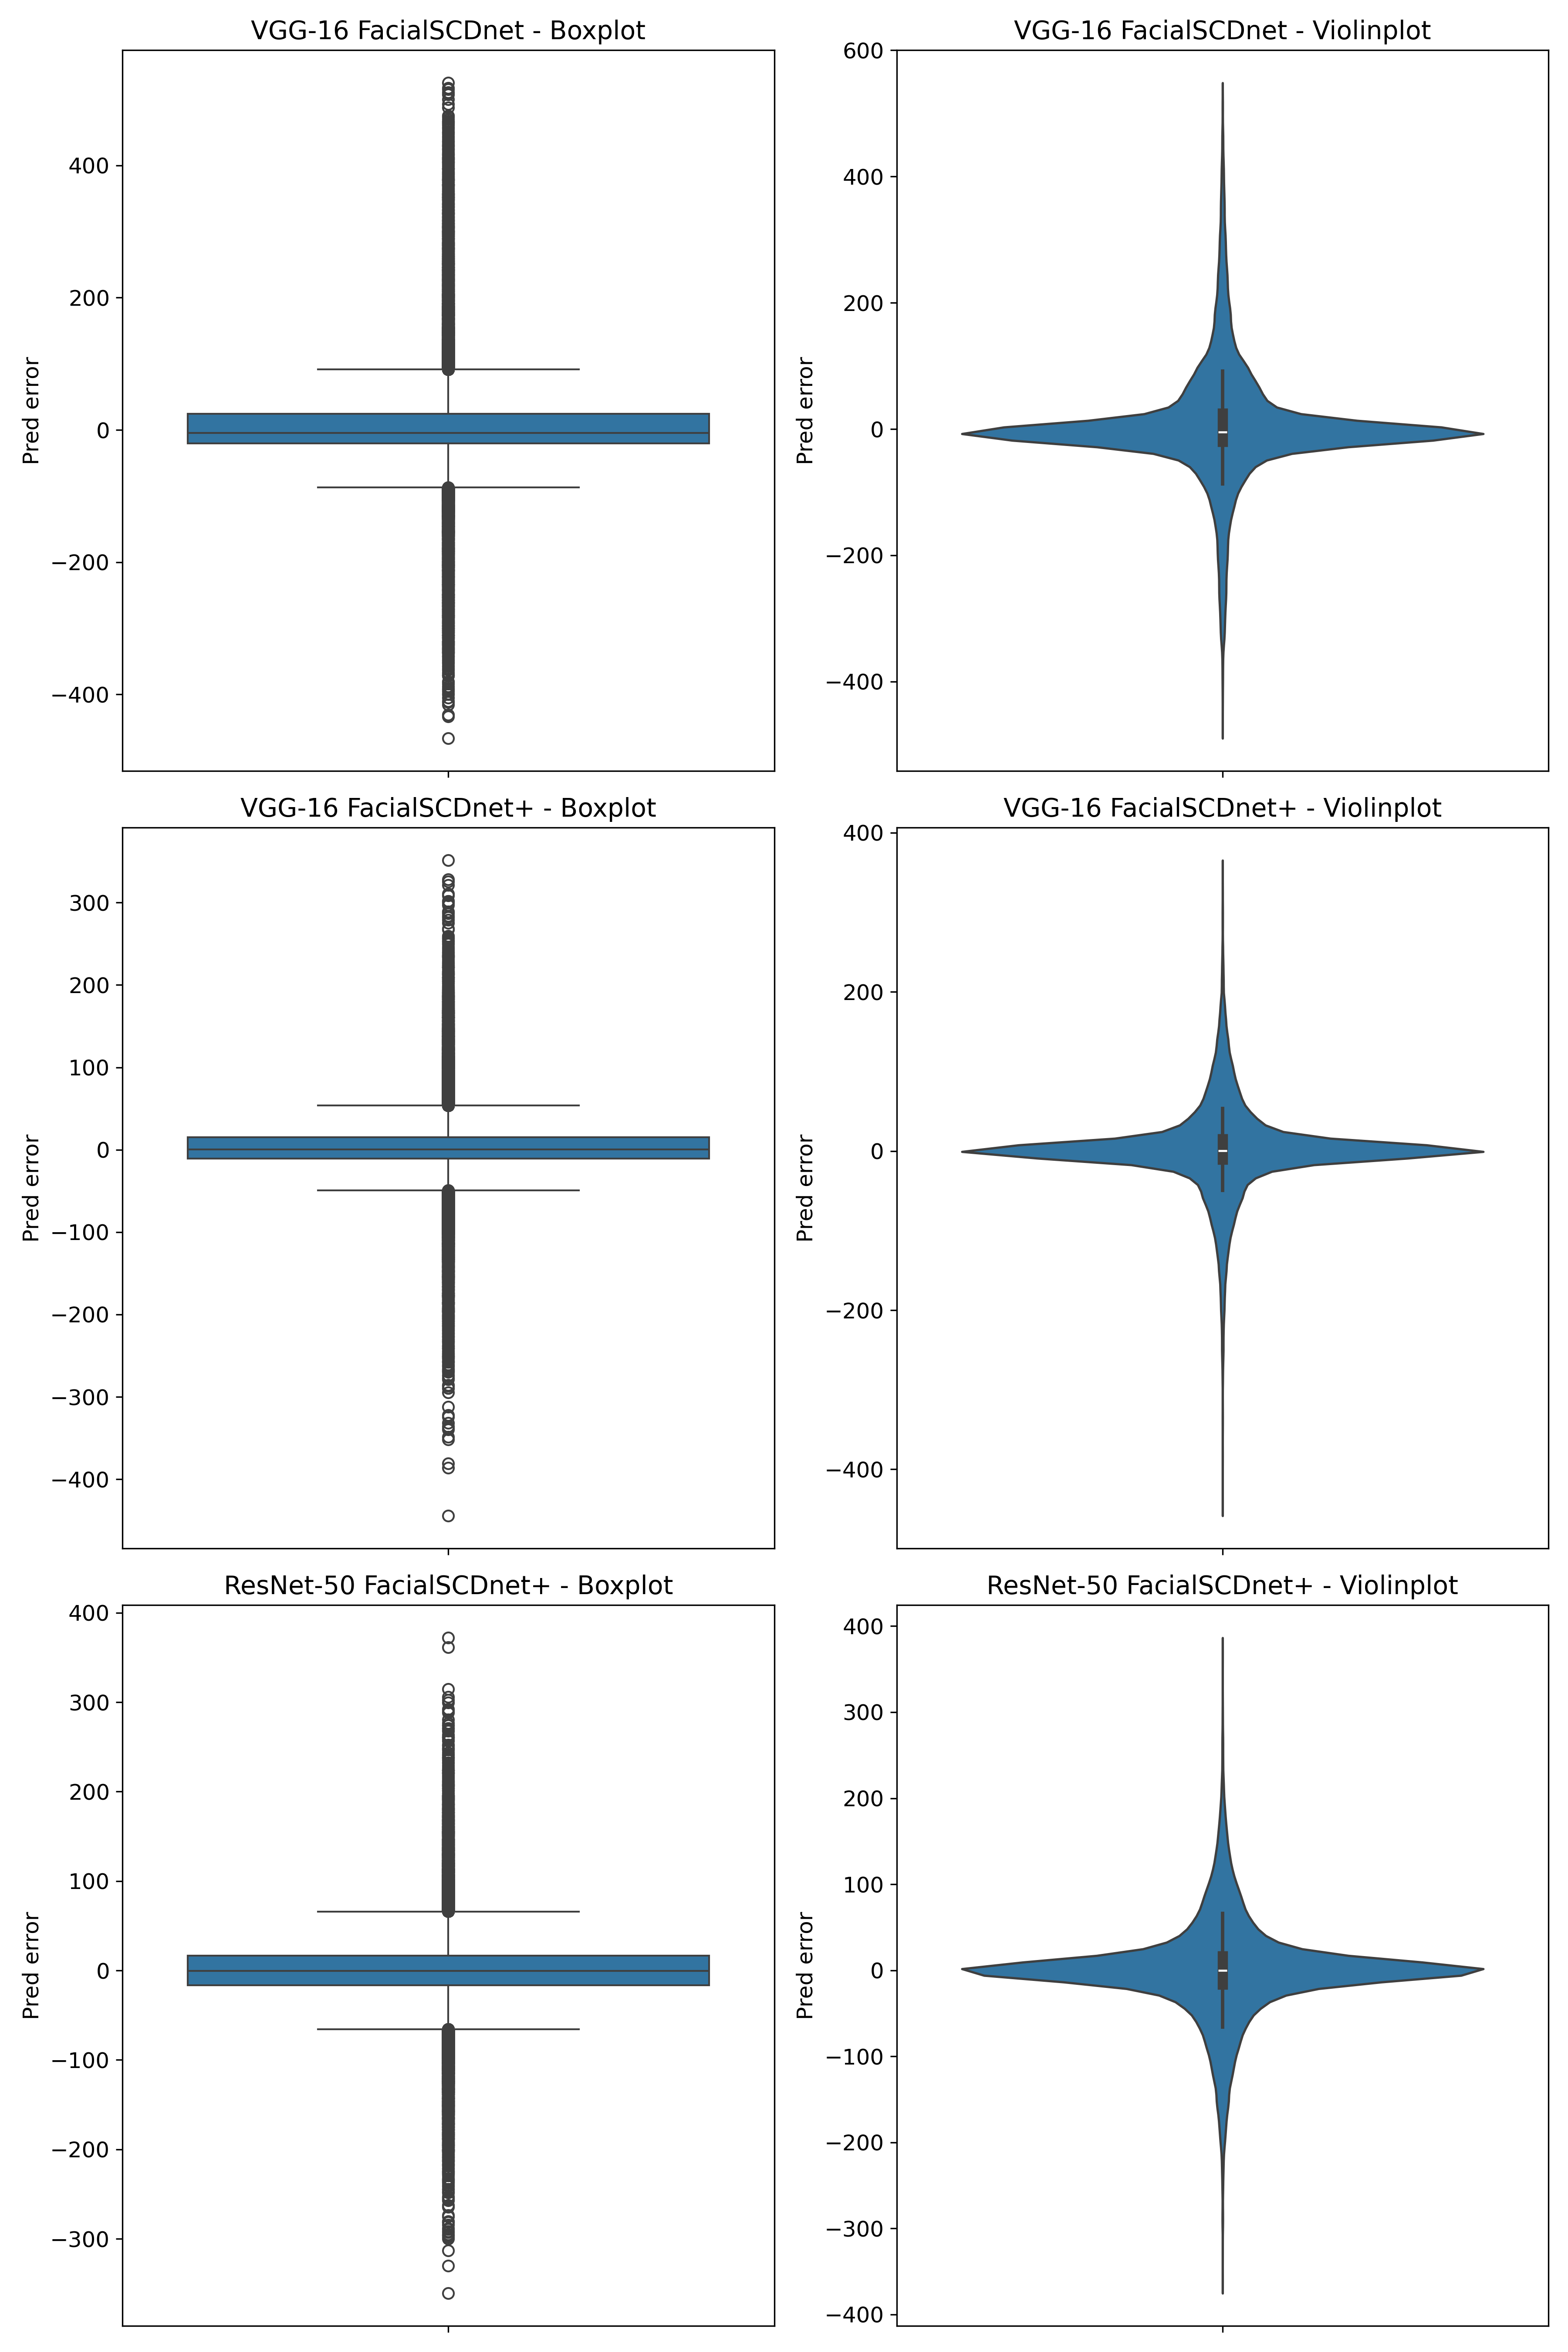
\includegraphics[width=\textwidth]{imagenes/cap5/boxplot_violinplot_comparison_own.png}
	\caption[Comparación predicciones de error test FacialSCDnet+.]{Gráfica que muestra la comparación de las predicciones de error para cada uno de los 3 modelos utilizados.}
	\label{fig33}
\end{figure}

En estas gráficas se puede observar cómo VGG-16 FacialSCDnet muestra la mayor variabilidad y la mayor cantidad de outliers, lo que sugiere que este modelo enfrenta más dificultades para hacer predicciones precisas en muchos casos. Los dos modelos de FacialSCDnet+ mejoran en comparación con FacialSCDnet, reduciendo tanto la variabilidad como la cantidad de outliers, lo que indica un desempeño más consistente. En particular, el modelo VGG-16 FacialSCDnet+ parece tener menor variabilidad, mientras que ResNet-50 presenta la menor cantidad de outliers.

\subsubsection{Test con imágenes reales}

Este conjunto de datos contiene 1134 imágenes reales en 29 distancias desde 50 a 500 cm. Los resultados de evaluar los modelos en este conjunto de datos se muestran en la Tabla \ref{test-real}.

\begin{table}[h]
	\centering
	\resizebox{\textwidth}{!}{%
	\begin{tabular}{lllll}
	\hline
	\begin{tabular}[c]{@{}l@{}}Métricas de \\ evaluación\end{tabular} &
	   &
	  \begin{tabular}[c]{@{}l@{}}VGG-16 \\ FacialSCDnet\end{tabular} &
	  \begin{tabular}[c]{@{}l@{}}VGG-16 \\ FacialSCDnet+\end{tabular} &
	  \begin{tabular}[c]{@{}l@{}}ResNet-50 \\ FacialSCDnet+\end{tabular} \\ \hline
	Distorsión &
	  \begin{tabular}[c]{@{}l@{}}Media (std)\\ Mediana\\ Mínimo\\ Perc 90\\ Perc 95\\ Perc 99\end{tabular} &
	  \begin{tabular}[c]{@{}l@{}}0.012 (0.016)\\ 0.008\\ 0.0\\ 0.03\\ 0.039\\ 0.084\end{tabular} &
	  \begin{tabular}[c]{@{}l@{}}0.007 (0.007)\\ 0.005\\ 0.0\\ 0.016\\ 0.022\\ 0.035\end{tabular} &
	  \begin{tabular}[c]{@{}l@{}}0.013 (0.01)\\ 0.011\\ 0.0\\ 0.026\\ 0.031\\ 0.041\end{tabular} \\ \hline
	MAE (cm) &
	  \begin{tabular}[c]{@{}l@{}}Media (std)\\ Mediana\\ Mínimo\\ Perc 90\\ Perc 95\\ Perc 99\end{tabular} &
	  \begin{tabular}[c]{@{}l@{}}31.594 (55.366)\\ 9.994\\ 0.04\\ 98.136\\ 154.061\\ 288.525\end{tabular} &
	  \begin{tabular}[c]{@{}l@{}}26.05 (48.391)\\ 8.69\\ 0.012\\ 71.072\\ 117.413\\ 261.572\end{tabular} &
	  \begin{tabular}[c]{@{}l@{}}39.852 (58.581)\\ 16.233\\ 0.018\\ 130.143\\ 179.454\\ 257.784\end{tabular} \\ \hline
	MRE (\%) &
	  \begin{tabular}[c]{@{}l@{}}Media (std)\\ Mediana\\ Mínimo\\ Perc 90\\ Perc 95\\ Perc 99\end{tabular} &
	  \begin{tabular}[c]{@{}l@{}}0.187 (0.33)\\ 0.103\\ 0.0\\ 0.409\\ 0.58\\ 1.61\end{tabular} &
	  \begin{tabular}[c]{@{}l@{}}0.098 (0.101)\\ 0.067\\ 0.0\\ 0.212\\ 0.3\\ 0.523\end{tabular} &
	  \begin{tabular}[c]{@{}l@{}}0.161 (0.126)\\ 0.137\\ 0.0\\ 0.342\\ 0.409\\ 0.523\end{tabular} \\ \hline
	\end{tabular}%
	}
	\caption[Métricas en el conjunto de test real de FacialSCDnet.]{Métricas en el conjunto de test real de FacialSCDnet, comparando los modelos VGG-16 y ResNet-50 de FacialSCDnet+ contra el modelo de FacialSCDnet.}
	\label{test-real}
\end{table}

Esta tabla refleja cómo VGG-16 FacialSCDnet+ presenta mejores resultados en todas las métricas, seguido por ResNet-50 FacialSCDnet+ y VGG-16 FacialSCDnet. Esto sugiere que el método FacialSCDnet+ proporciona una mejora significativa en el rendimiento de la predicción en comparación con el método FacialSCDnet estándar, y que el modelo VGG-16 es más efectivo que el ResNet-50 en este contexto específico.

En este contexto, es notable destacar un error cometido en el método FacialSCDnet. A la hora de evaluar el modelo con las imágenes reales, se les aplicaba una máscara para añadirles un fondo sintético. Esto provocaba que el rendimiento del modelo aumentara considerablemente. Sin embargo, se estaba cometiendo un sesgo significativo debido a la adición de estos fondos. Estos resultados se pueden ver en el artículo de FacialSCDnet \cite{14}.

La siguiente gráfica (Figura \ref{fig34}) muestra los valores predichos frente a los valores objetivos para cada uno de los 3 modelos utilizados. La línea roja discontinua representa la línea de referencia donde las predicciones coincidirían perfectamente con las etiquetas objetivo. 

\begin{figure}[h]
	\centering
	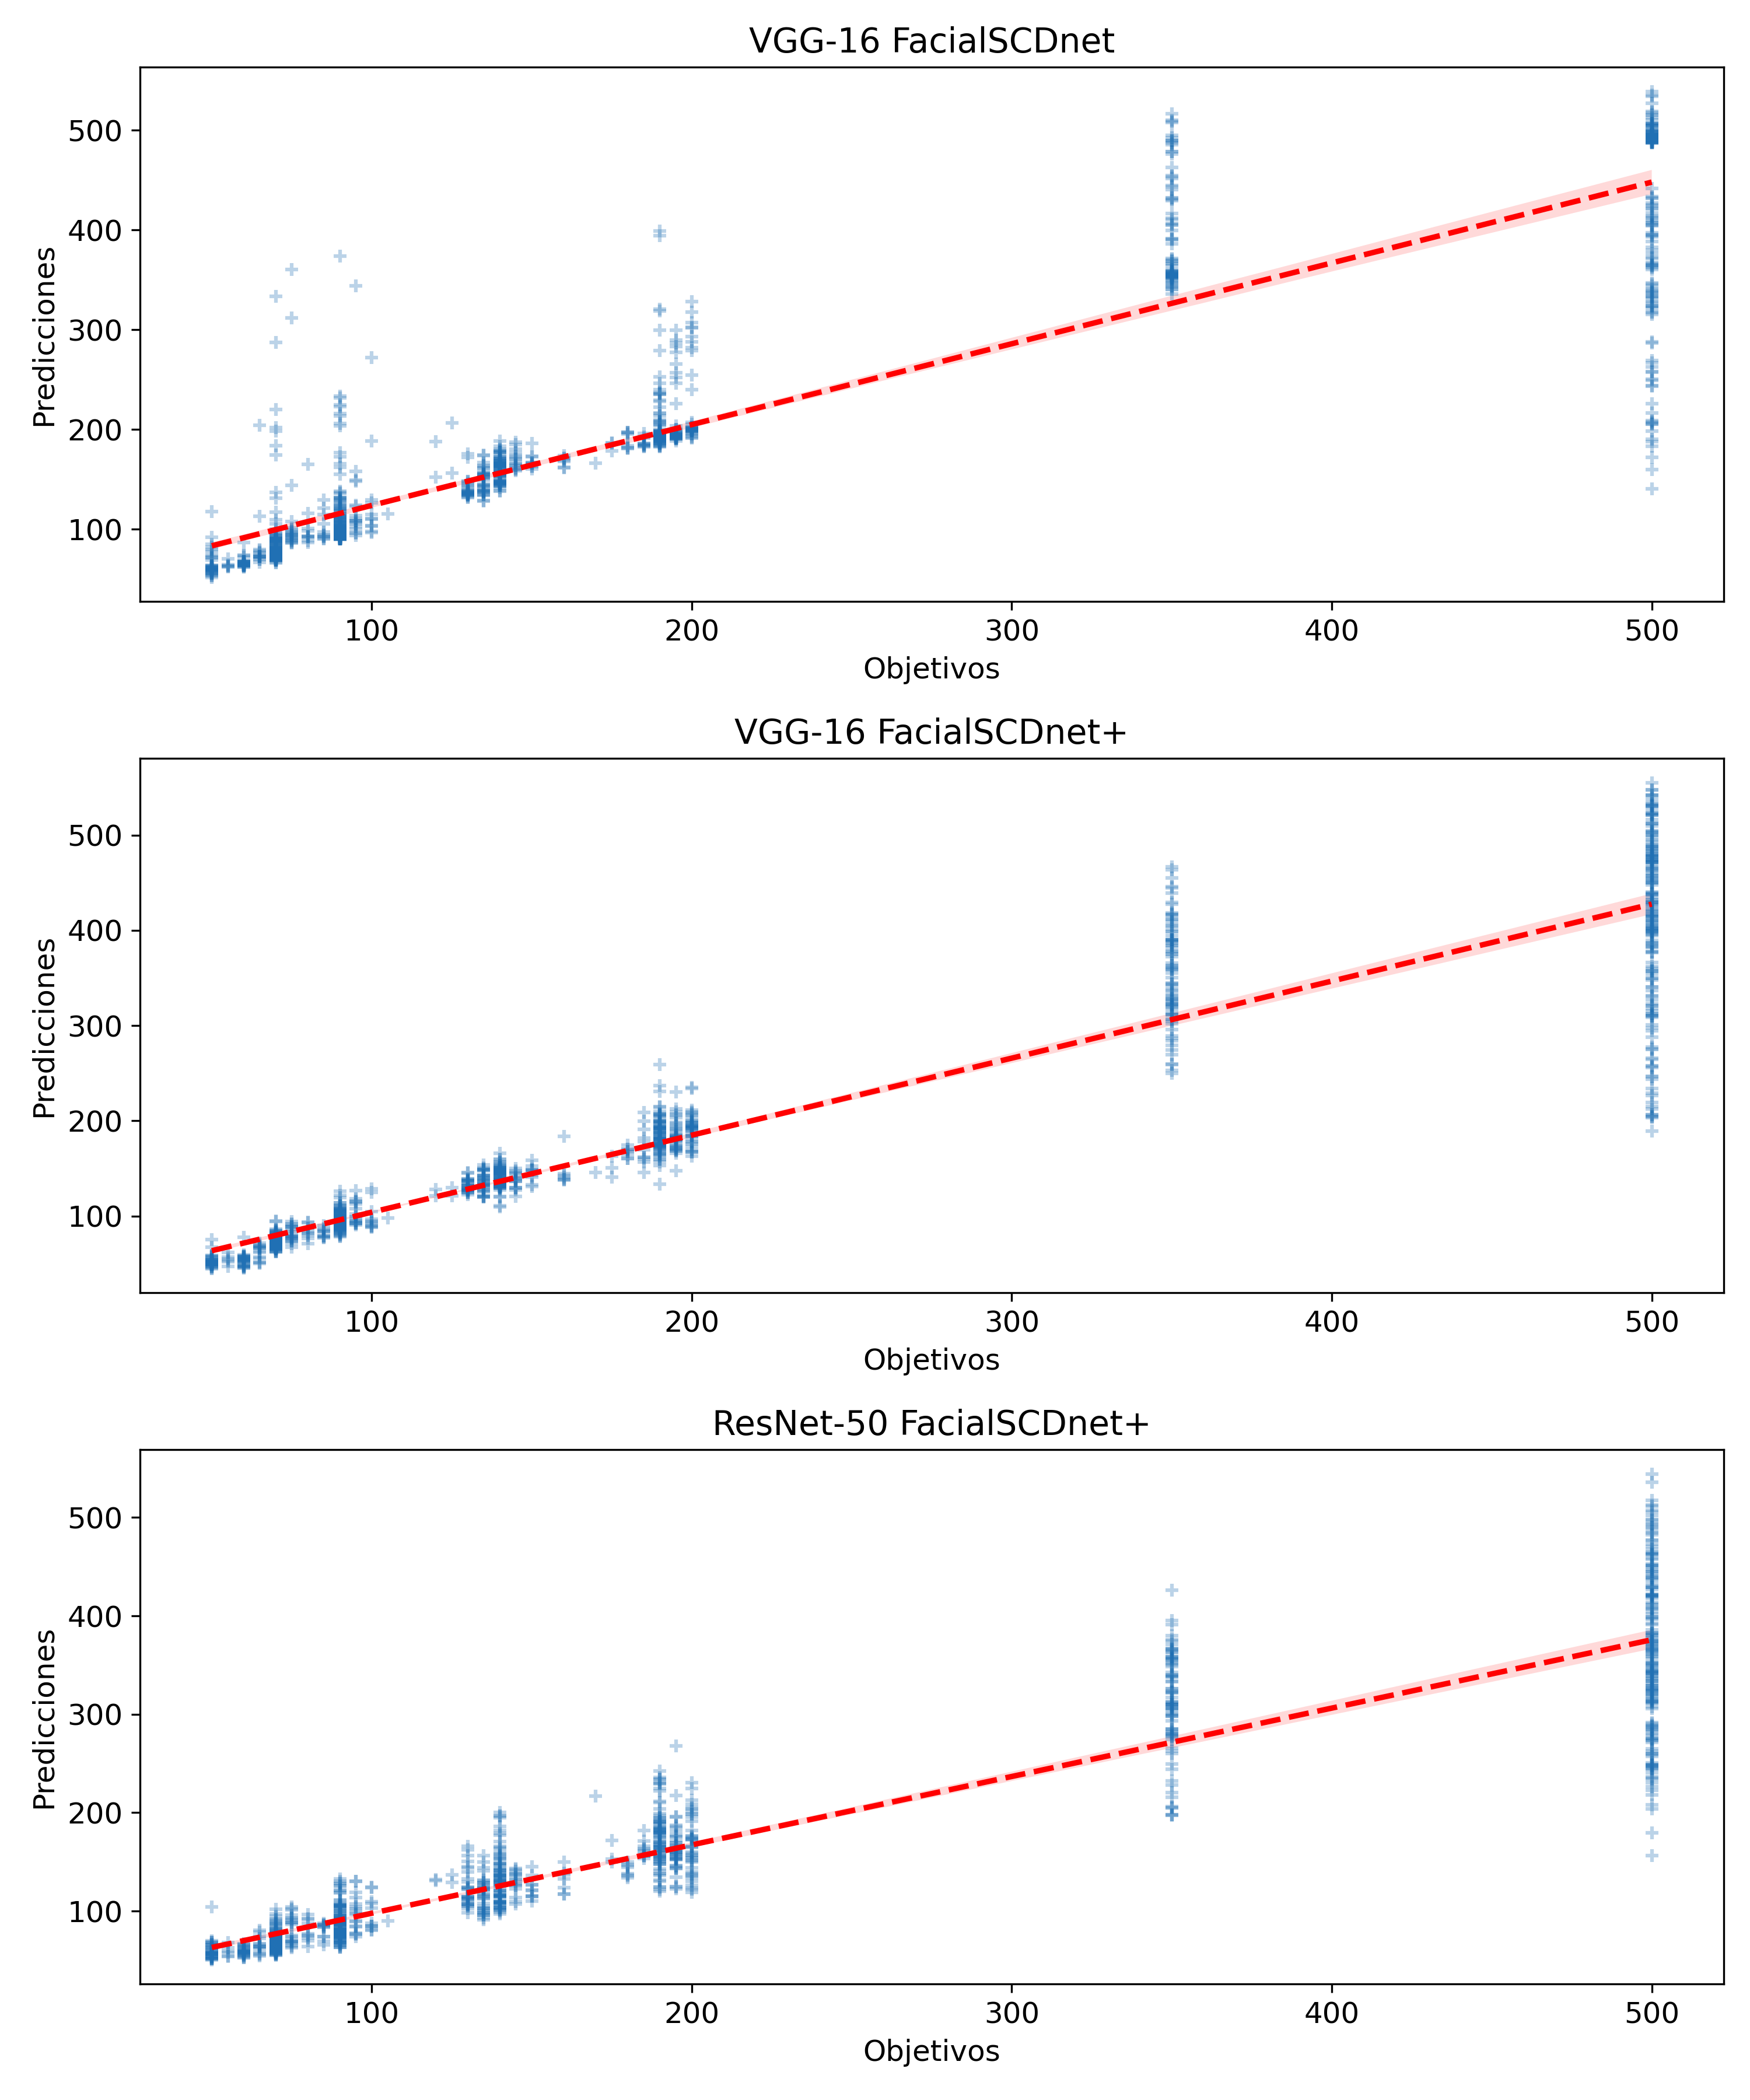
\includegraphics[width=\textwidth]{imagenes/cap5/comp_etiquetas_real.png}
	\caption[Comparación etiquetas test FacialSCDnet.]{Gráfica que muestra la comparación de etiquetas predichas vs las etiquetas objetivo para cada uno de los 3 modelos utilizados.}
	\label{fig34}
\end{figure}

Se puede observar como en el modelo VGG-16 FacialSCDnet, las predicciones son menos precisas en general, especialmente en valores más altos, donde se observa una mayor dispersión. En cambio, los modelos de FacialSCDnet+ presentan un mejor desempeño. Específicamente, el modelo VGG-16 FacialSCDnet+ muestra una mayor precisión en las predicciones tanto para valores bajos como para valores altos, comparado con el VGG-16 FacialSCDnet. Por su parte, el modelo ResNet-50 FacialSCDnet+ también demuestra un alto grado de precisión, aunque con una ligera tendencia a sobrestimar algunos valores altos. 

La figura \ref{fig35} muestra una comparación de las predicciones de error para los tres modelos utilizando tanto gráficos de caja como gráficos de violín.

\begin{figure}[h]
	\centering
	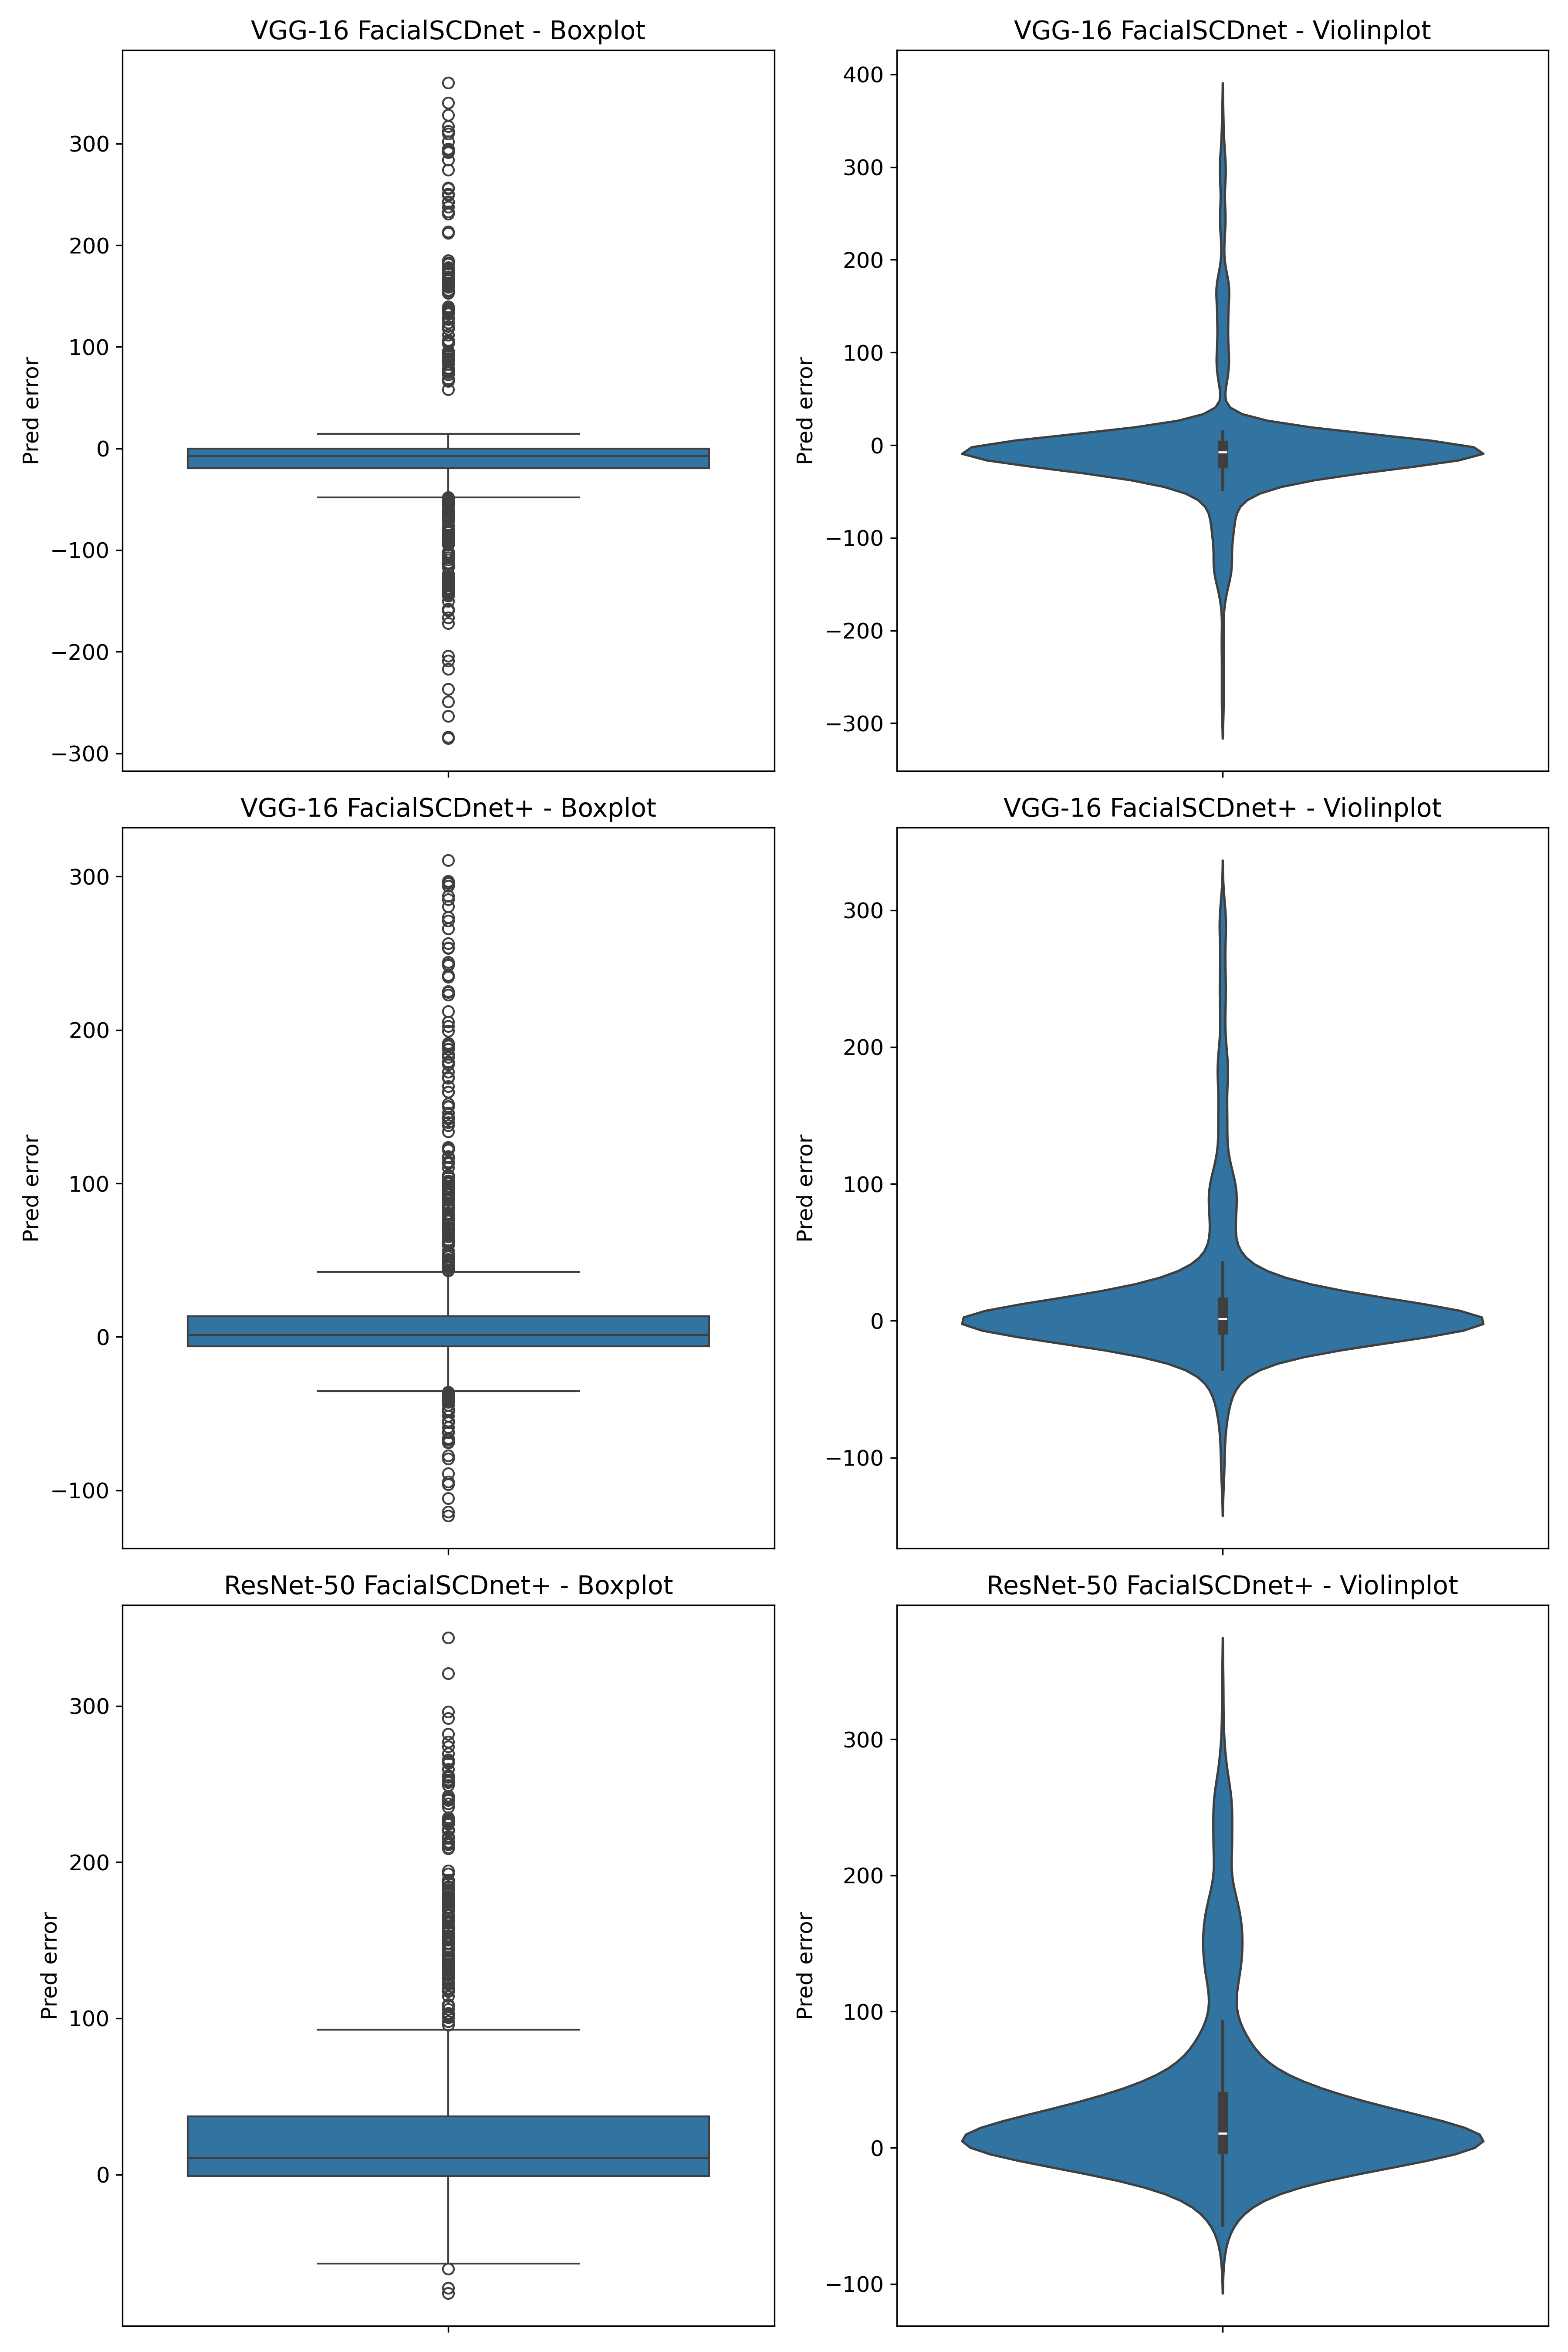
\includegraphics[width=\textwidth]{imagenes/cap5/boxplot_violinplot_comparison_real.png}
	\caption[Comparación predicciones de error test FacialSCDnet.]{Gráfica que muestra la comparación de las predicciones de error para cada uno de los 3 modelos utilizados.}
	\label{fig35}
\end{figure}

Se observa que VGG-16 FacialSCDnet presenta la mayor cantidad de outliers, lo que sugiere que este modelo tiene más dificultades para hacer predicciones precisas en ciertos casos. Además, este modelo tiende tanto a sobreestimar como a infraestimar las predicciones. Por otro lado, ambos modelos de FacialSCDnet+ muestran una menor cantidad de outliers, aunque tienen una mayor variabilidad, especialmente el ResNet-50 FacialSCDnet+. El modelo VGG-16 FacialSCDnet+, a pesar de tener una variabilidad ligeramente mayor que el VGG-16 FacialSCDnet, presenta menos outliers, lo cual sugiere que es el modelo más consistente de los presentados.